\documentclass[main.tex]{subfiles}
\begin{document}
	\chapter{Organization}
	\chapterauthor{Marc Stelter, Torge Olliges}
	\label{organisation}
	
	\section{Schedule}
	The project ran from the 13.10.2019 to 31.05.2020. During this time window the following dates have been set:
	\begin{itemize}
		\item 20.12.2019 Milestone 1: Get used to the new technologies and develop a minimal running setup.
		\item 06.03.2020 Milestone 2: Finish a working setup for the tasks grocery storing and clean up
		\item Early April 2020: Project day Uni Bremen
		\item End of April 2020: RoboCup German Open
		\item 08.05.2020: Milestone 3: End of Development
		\item 31.05.2020: Due date Project documentation
	\end{itemize} 

	\section{Model of Development}
	\label{sec:modelofdevelopment}
	The model of development is a custom \href{http://projektmanagement-definitionen.de/glossar/scrum/}{scrum} variation. Scrum itself is an agile project management framework. It is an iterative and incremental model meaning that the actual product is developed during different iterations each ending with a prototype, which is then used as a base for the next iteration. Allowing the final product to grow step by step and leaving room for adjustments during implementation. Each iteration is called a sprint and lasts 30 days. For each sprint, tasks are taken from a product backlog and added to the sprint backlog. Also, there exists daily meetings meant to update each member of the current progress and problems. Scrum also defines several roles. Like a product owner, development team, scrum master besides others.  
	
	It has already been mentioned that the original scrum model has been altered for this project. Sprints no longer have a fixed length of 30 days. Instead, a variable length of 7, 14, or 21 days could be defined at the start of each sprint depending on the complexity of the next increment. Since the project is not a full-time project with each member working daily on it the daily stand-ups have been replaced by a stand up on Wednesday and Friday. 
	
	Also, a weekly meeting was scheduled for each Friday to discuss the current progress, problems, and possible features with the tutors.
	
	To keep track of the tasks a \href{https://www.atlassian.com/de/agile/kanban/boards}{Kanban board} in the form of \href{https://trello.com/de}{Trello} was used. A Kanban board is a tool allowing the visualization of the workflow. The tasks are represented by a card sorted into different columns each representing a state in the workflow. Once a task moves from one state to another it is forwarded to the corresponding column.
	
	The following figure \ref{developmentmodel}	shows the used version of the scrum model.
	
	\begin{figure}[h]
		\centering
		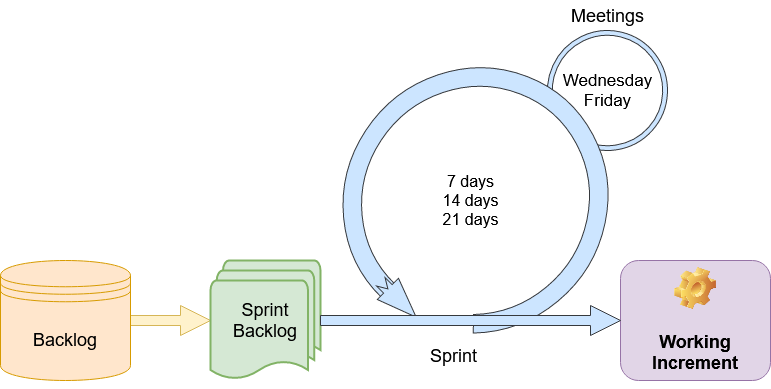
\includegraphics[width=0.85\textwidth]{pictures/diagramms/Development-model.png}
		\caption{Development Model}
		\label{developmentmodel}
	\end{figure}

	\section{Roles}
	The roles were assigned for each milestone, it was assured that each person held at least two roles throughout the project. The roles have been assigned as follows:
	\begin{itemize}
		\item Scrum master / Project leader: Organizing plenum and sprints. Push decision making.
		\item Product owner: Take care of the backlog
		\item Kanban master: Takes care of the Kanban board
		\item Foreign minister: External representation and organization of project day. The foreign minister role is excluded from the milestone role changes.
		\item Group leader: Organization of the expert groups, leading and preparing the weekly meetings.
		\item Quality assessment: check documents and code for errors.
	\end{itemize}
	
	\section{Software}
	The following applications or services have been used in the organization of the project:
	\begin{itemize}
		\item \href{https://www.microsoft.com/de-de/microsoft-365/microsoft-teams/group-chat-software}{Microsoft teams}: Chat interaction, wiki, protocols, presentations.
		\item \href{https://trello.com/de}{Trello}: Kanban board
		\item \href{https://github.com/}{Github}: Repository for the project code
		\item \href{https://jitsi.org/}{Jitsi}: Online conference tool
		\item \href{https://discord.com/}{Discord}: Online communication tool
		\item \href{https://app.diagrams.net/}{Draw.io}: Online tool for creating diagrams 
	\end{itemize}  

	\section{Corona}
	Due to the outbreak of the Coronavirus and the following regulations access to the HSR was no longer possible as of 16.03.2020. Therefore the following development has been done with the gazebo simulator.
	The meetings have been carried out via \textit{Jitsi} and \textit{Discord}. An additional project computer has been provided to run the simulation.
	The project day and RoboCup have been canceled.
	
\end{document}

